\documentclass[12pt]{book}

\usepackage[a4paper, portrait, margin=0.75in]{geometry}
\usepackage{graphicx} % Required for inserting images
\usepackage[page,toc,titletoc,title]{appendix}
\usepackage{mathptmx}
\usepackage{pdflscape}
\usepackage{pdfpages}
\usepackage{enumitem}
\usepackage{hyperref}
\usepackage{cleveref}

\title{Integrating streamed sensor data into a distributed model of a complex system \\
\large{A report submitted in partial fulfilment of the requirements for the degree of \\
\textbf{Bachelor of Engineering (Hons) in Software Engineering} \\
at \\
\textbf{the University of Waikato}
}}

\author{Bert Downs  \\ 
Supervised by Tim Walmsley, Mark Apperley }

\date{October 2024}

\begin{document}

\maketitle


\chapter*{Abstract}

Modern factories are equipped with a variety of sensors that monitor the state of the factory and products. To fully utilise this sensor data, the field of Digital Twinning is emerging, which combines live factory data, historical state, and a model of the factory to predict future states. The process of creating a digital twin lacks standardization. This project develops a standardised framework for creating digital twins of chemical plants, using the Ahuora Digital Twin Platform and industry standard data processing tools. 

% TODO: Something about results and evaluation stuff.

\tableofcontents

\newpage


\chapter{Introduction}


\section{Background}

`Project Ahuora' is a Ministry of Business, Innovation and Employment (MBIE) funded project that aims to decarbonise the process heat sector. 
By decarbonising, New Zealands' greenhouse gas emissions will be reduced. Cost savings from reduced energy consumption are anticipated, along with increased energy independence.
This is a multi-disciplinary project that involves researchers from the University of Waikato, University of Auckland, Massey University,
and other global universities. Chemical Engineers bring understanding of the chemical processes that are used in industry. Electrical Engineers bring understanding of the grid system
and how to integrate renewable energy sources. Mechanical engineers bring understanding of how to design and build more efficient systems. Software Engineers bring understanding of how to
model, simulate, and monitor complex systems. 

A key objective is to develop a digital twin platform for the chemical processing industry. This platform will allow New Zealand factory operators to model their processes, simulate different scenarios, and monitor their processes in real-time.
This will enable factory operators to make data-driven and scientifically backed decisions on how to improve their processes. A digital twin can recognise where the factory is underperforming, suggest real-time improvements, and help plain future investments.  


\section{Motivation}

Currently, Ahuora has developed a Web-based simulation platform that allows users to create a digital twin of their factory. 
This platform is based on steady-state simulation, which simulates a factory at a single point in time. All factory conditions are manually specified by the user.
This platform is useful for modelling changes to a factory before construction, or understanding the factory's performance under different conditions.
However, it cannot be considered a ``Digital Twin'' because it does not take into account the factory's real-time state.
By integrating real-time sensor data into the simulation, the platform can monitor the factories' performance, and suggest tunings that will optimise resource efficiency.
The data can also be used to predict and avoid failures and downtime, a key problem where many resources are wasted.
Additionally, models created in the Ahuora Simulation Platform during the design phase could also be used during operation, minimising overhead costs.

Including real-time data in the simulation is needed to improve the usefulness of the Ahuora Platform in industry. 
The system needs to meet industry requirements for security, scalability, and reliability. As such, this project 
has been commissioned to develop a standardised framework to enable the integration of real-time sensor data into the Ahuora Digital Twin Platform.

% Todo: Include a substantial section explaining the Ahuora Digital Twin Platform, and what it does. THis is a necessary background for the project. The marker won't understand otherwise.

\section{Objectives}

The objectives of this project are as follows:
\begin{itemize}
    \item Conduct a literature review on Digital Twins, Digital Twin Platforms, and Data Processing Tools.
    \item Conduct an Exploratory Analysis of techniques and tools for digital twin development, based on their applicability to the Ahuora Digital Twin Platform and the requirements of live data processing.
    \item Develop the Ahuora Digital Twin platform to a stage where support for live data processing can be added.
    \item Develop a standardised framework for integrating real-time sensor data into the Ahuora Digital Twin Platform.
    \item Develop a prototype implementation of the framework.
    \item Evaluate the prototype implementation in a case study.
    \item Identify areas for future work.
\end{itemize}
\section{Scope}

Full integration of real-time sensor data into the Ahuora Digital Twin Platform is out of scope for this project. 
This project will focus on identifying techniques and tools for simulation and modelling that will be needed in a industry setting,
and developing a prototype live data processing system for Ahuora that is extensible enough to support those techniques and tools.

\section{Structure of the Report}

\chapter{Literature Review}

\section{Digital Twins}

\section{Digital Twin Platforms}

\section{Data Processing Tools}

\chapter{Methodology}

This project was conducted as part of a real-world, collaborative effort to build the Ahuora Digital Twin platform, so the methodology followed engineering principles, rather than being purely academic experimentation. Research into live data processing techniques could only be conducted as far as the Digital Twin Platform supported them. The focus of the project moved between improving the Simulation Platform to support more modelling techniques, and developing a live data processing system that could be integrated into the platform.

\section{Experimentation in IDAES}

The Ahuora Digital Twin Platform is built on top of the IDAES Process Systems Engineering Framework. Because of this, the IDAES framework was used as a testbed for experimentation with live data processing techniques. The IDAES framework is a Python library that provides tools for modelling and simulating chemical processes. It is designed to be extensible, so that new modelling techniques can be added to it. 


From the Literature Review, a variety of modelling techniques were identified, including Dynamic Modelling, Surrogate Modelling, and Optimisation. The Ahuora Digital Twin platform is currently based on steady-state simulation and does not support these techniques. The IDAES framework was used to test the feasibility of integrating live data processing techniques into the Ahuora Digital Twin Platform.


\subsection{Dynamic Modelling}

I used the IDAES framework to develop a dynamic model of a steam tank, with a valve controlling the inlet and outlet pressure and flow rate. A PID controller was used to control the valve opening fraction to regulate the pressure in the tank.

\begin{figure}
    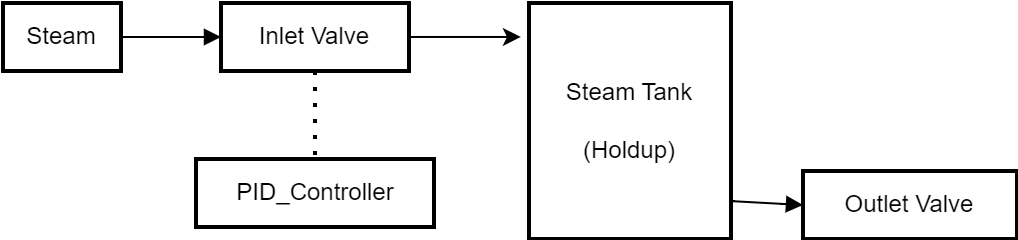
\includegraphics[width=0.9\textwidth]{dynamicmodelling.png}
    \caption{Dynamic Modelling of a Steam Tank}
    \label{fig:dynamicmodelling}
\end{figure}

This provided a simple example of a dynamic system. The inlet and outlet valve and the PID controller were not dynamic models: From a mathematical perspective, this means their properties were fully determined by the inlet and outlet conditions. The only dynamic model was the Steam Tank. From a mathematical perspective, this means that the state of the steam tank was determined by the inlet and outlet conditions, but also the previous state of the tank, i.e how "full" the tank is.


\subsubsection{Key Findings}

\begin{itemize}
    \item The IDAES framework is well-suited to dynamic modelling, as it provides tools for creating and solving differential equations. It can easily model the same system at different time scales.
    \item The Ahuora Simulation Platform will require substantial changes to support dynamic modelling. Rather than storing a single value for each property, it will need to store the state of each property at each time step.
    \item This will also require significant UI changes to view the state of the system at different time steps. This could be achieved through some sort of time slider, and graph visualisations of properties over time.
    \item Specifying the initial conditions of the system will be more complex, as the user will need to specify the initial state of dynamic properties, such as the initial tank level. Other properties, such as the valve opening fraction, will need to be specified as functions of time.
\end{itemize}

\subsection*{Surrogate Modelling}

Surrogate Modelling is the process of creating a simplified model of a complex system. This is usually done using machine learning techniques. This provides a good test case of implementing data-driven modelling techniques in the IDAES framework.

\subsubsection{Key Findings}
\begin{itemize}
    \item Surrogate Modelling may be achieved using IDAES's built-in PySMO libraries, or other similar libraries such as OMLT. It is reasonably straightforward to train a surrogate model on non-dynamic
\end{itemize}

\subsection*{Optimisation and Control}




\section{Prototype Development}

\section{Minimum Viable Product}

\section{Extensions}

\section{Future Work}

\chapter{Case Study: Heat Pump Dryer}

\section{Motivation}

\section{Method}

\section{Results}

\section{Discussion}

\chapter{Conclusion}

\chapter{References}

\bibliographystyle{unsrt} % We choose the "plain" reference style
\bibliography{refs} % Entries are in the refs.bib file

\begin{appendices}



% \chapter{Project Proposal} \label{sec:proposal}
% The project proposal is included as an appendix on the following page.


% 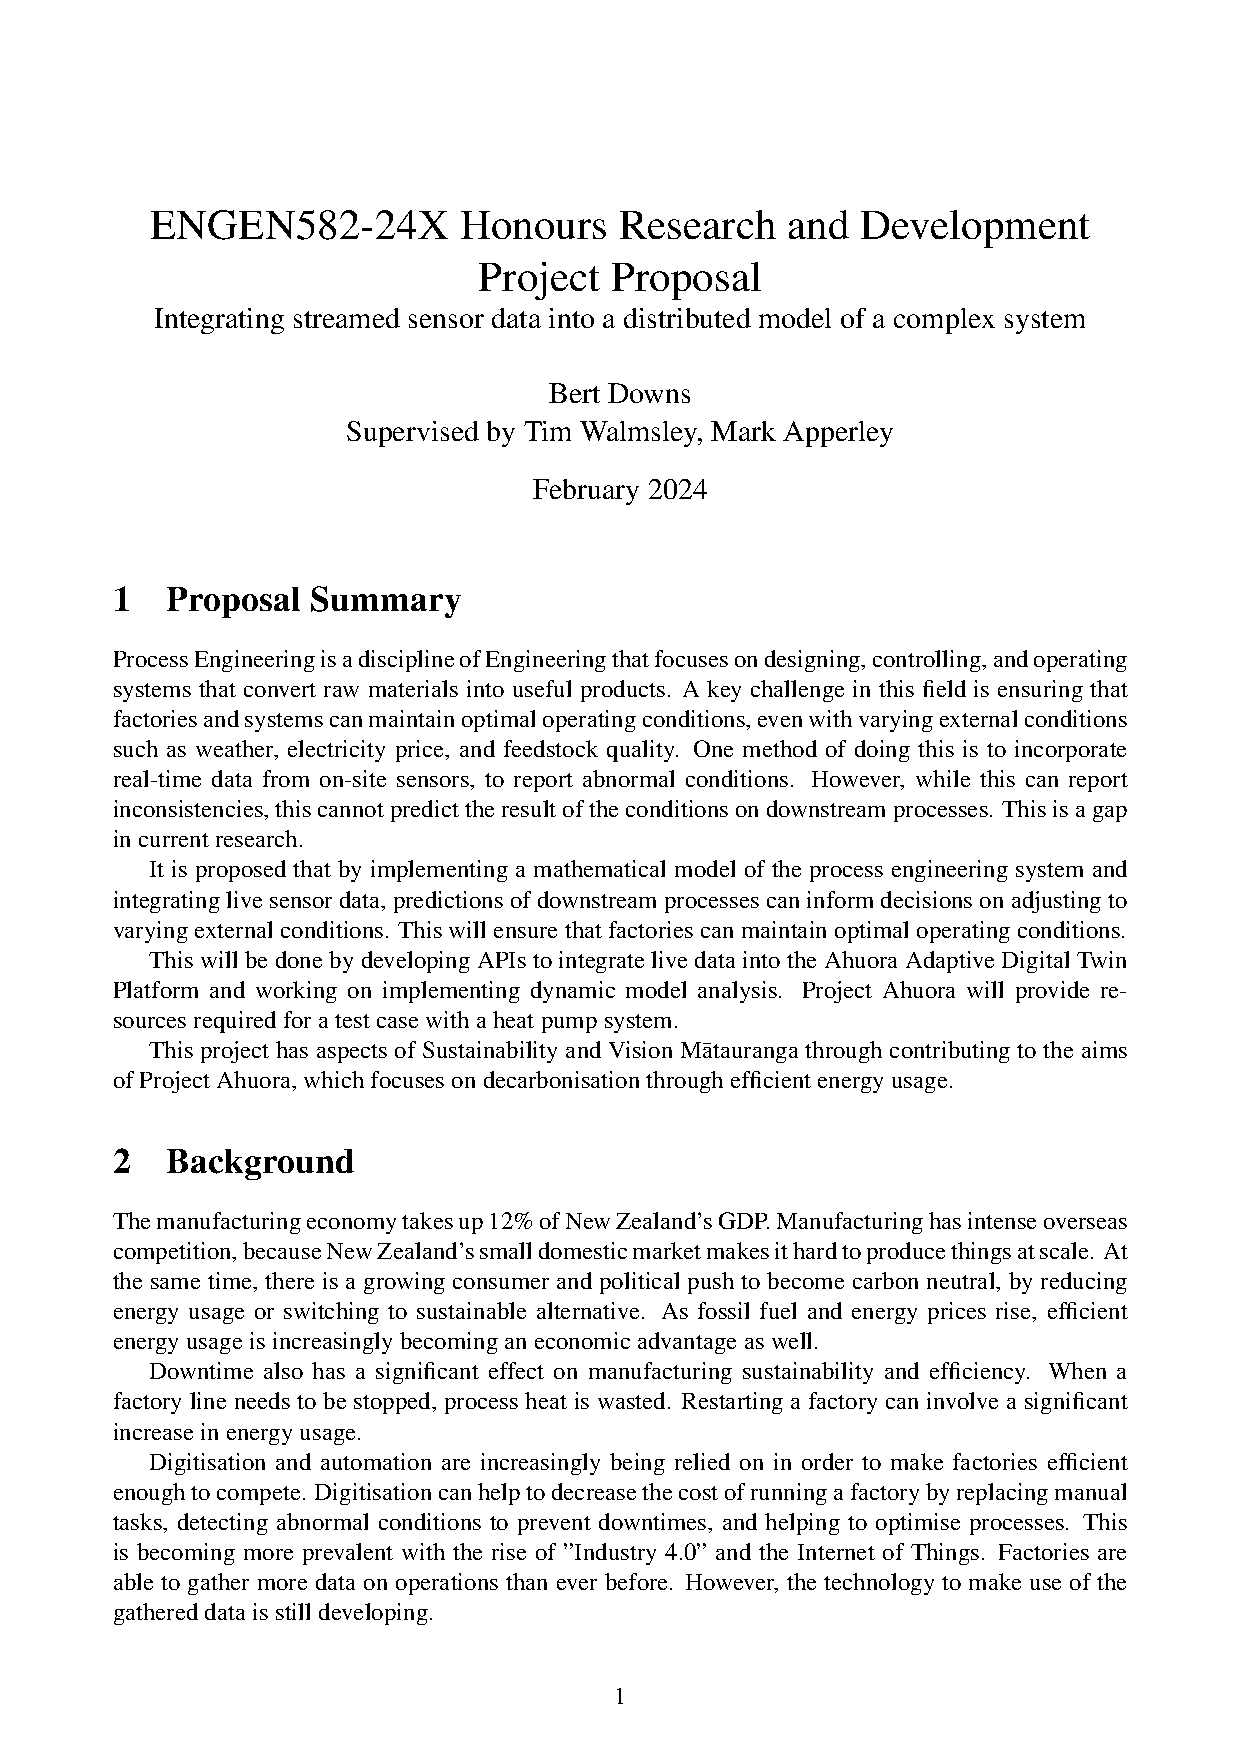
\includepdf[pages=1-4]{proposal.pdf}

% \begin{landscape}
%     \includepdf[pages=5,angle=90]{proposal.pdf}
% \end{landscape}

% \chapter{Literature Review} \label{sec:litreview}
% The literature review is included as an appendix on the following page.

% 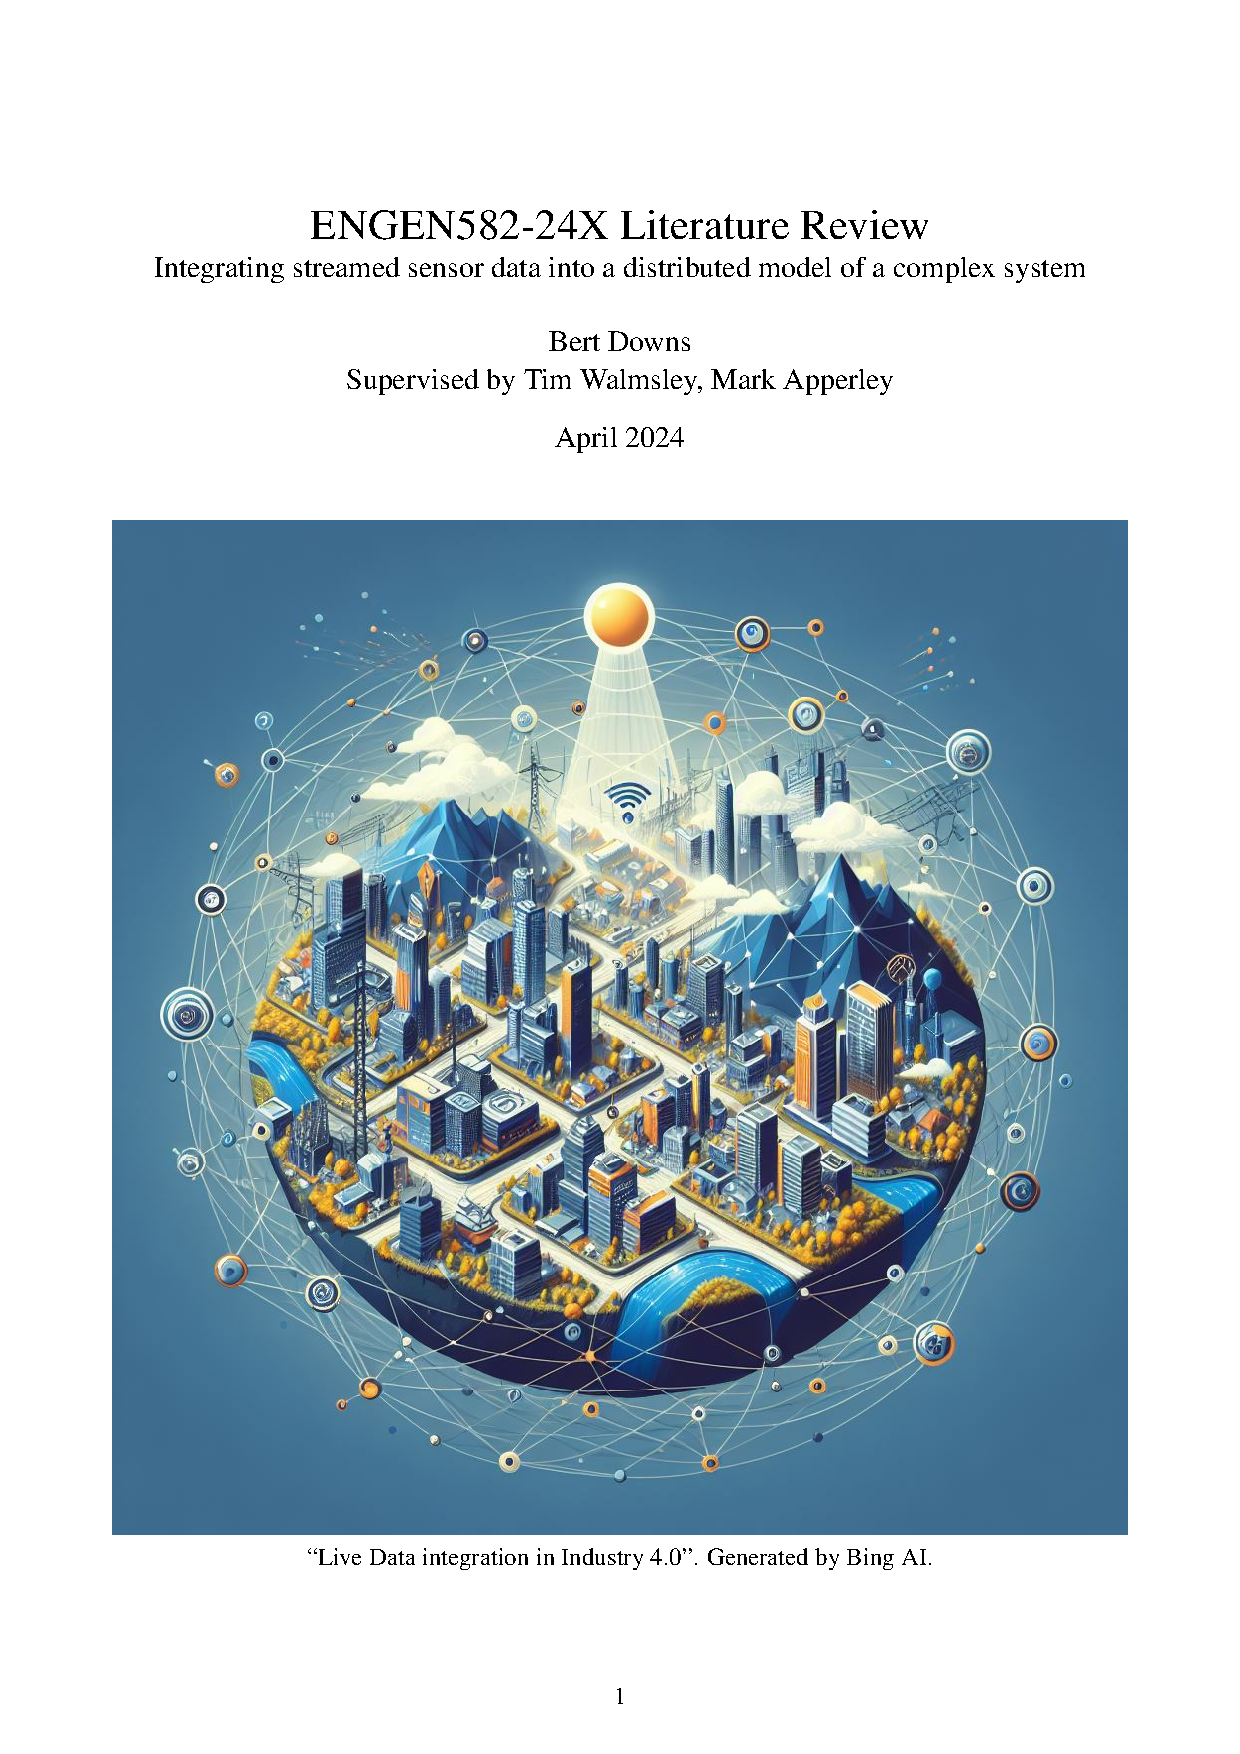
\includepdf[pages=-]{literature_review.pdf}

\end{appendices}
\end{document}